\noindent
Machine learning techniques are becoming increasingly important for many data-analytics models, and healtcare data analyis is no exception. The machine learning algorithms typically operate on data in the form of a matrix where e.g. rows correspond to features and columns correspond to samples. Thus, the problem in our settings is to protect a machine learning algorithm from an adversary who seeks to gain an information about the data from algorithm's output by perturbing the value in an element of the training data matrix. Despite the fact that random noise adding mechanism has been widely studied in privacy-preserving machine learning, there remains the challenge of studying privacy-utility trade-off for matrix-valued query functions. Our recent work~\cite{Kumar/IWCFS2019} has suggested a novel entropy based approach for resolving the privacy-utility trade-off for real-valued data matrices. The study in~\cite{Kumar/IWCFS2019} derives mathematically the probability density function of noise that minimizes the expected noise magnitude together with satisfying the sufficient conditions for $(\epsilon,\delta)-$differential privacy. This text shows that the optimal noise adding mechanism results in the magnitude of noise a multi-fold reduction (up to several tens times) over the classical Gaussian mechanism. Further, the optimal noise adding mechanism is applied for privacy-preserving distributed learning of deep models.  

%Consider a data-set consisting of $N$ number of samples with each sample having $p$ number of attributes represented by a matrix $\mathrm{Y} \in \mathbb{R}^{p \times N}$. A given machine learning algorithm, training a model using data matrix $\mathrm{Y}$, can be represented by a mapping, $\mathcal{A}: \mathbb{R}^{p \times N} %\rightarrow \mathbf{M}$, where $\mathbf{M}$ is the model space.  
%\begin{definition}[A Private Algorithm]\label{definition_private_algorithm}
%Let $\mathcal{A}^+ : \mathbb{R}^{p \times N} \rightarrow Range(\mathcal{A}^+)$ be a mapping defined as
%\begin{IEEEeqnarray}{rCl}
%\mathcal{A}^+\left(\mathrm{Y}\right) & = & \mathcal{A}\left(\mathrm{Y} + \mathrm{V}\right),\;  \mathrm{V} \in %\mathbb{R}^{p \times N}
%\end{IEEEeqnarray}  
%where $\mathrm{V}$ is a random noise matrix with $f_{\mathrm{v}_j^i}(v)$ being the probability density function of its $(j,i)-$th element $\mathrm{v}_j^i$; $\mathrm{v}_j^i$ and $\mathrm{v}_j^{i^{\prime}}$ are independent from each other for $i \neq i^{\prime}$; and $\mathcal{A}: \mathbb{R}^{p \times N} \rightarrow \mathbf{M}$ (where $\mathbf{M}$ is the model space) is a given mapping representing a machine learning algorithm. 
%\end{definition}  
%\begin{definition}[$d-$Adjacency for Data Matrices]\label{def_adjacency_matrices}
%Two matrices $\mathrm{Y},\mathrm{Y}^{\prime} \in \mathbb{R}^{p \times N}$ are $d-$adjacent if for a given $d  \in \mathbb{R}_{+}$, there exist $i_0 \in \{1,2,\cdots,N\}$ and $j_0 \in \{1,2,\cdots,p\}$ such that $\forall i \in \{1,2,\cdots,N\}, j \in \{1,2,\cdots,p\}$,
% \begin{IEEEeqnarray*}{rCl}
%\left | \mathrm{y}^i_j - \mathrm{y}^{\prime i}_j \right | & \leq & \left\{ \begin{array}{cc}
%d, & \mbox{if $i = i_0,j = j_0$} \\
%0, & \mbox{otherwise}
%  \end{array} \right.
%\end{IEEEeqnarray*}    
%where $\mathrm{y}^i_j$ and $\mathrm{y}^{\prime i}_j$ denote the $(j,i)-$th element of $\mathrm{Y}$ and $\mathrm{Y}^{\prime}$ respectively. Thus, $\mathrm{Y}$ and $\mathrm{Y}^{\prime}$ differ by only one element and the magnitude of the difference is upper bounded by $d$. 
%\end{definition} 
%\begin{definition}[$(\epsilon,\delta)-$Differential Privacy for %$\mathcal{A}^+$]\label{def_differential_privacy}
%The algorithm $\mathcal{A}^+\left(\mathrm{Y}\right)$ is $(\epsilon,\delta)-$differentially private if
% \begin{IEEEeqnarray}{rCl}
%\label{eq_differential_privacy}  Pr\{ \mathcal{A}^+\left(\mathrm{Y}\right) \in \mathcal{O} \} & \leq & \exp(\epsilon) Pr\{ \mathcal{A}^+\left(\mathrm{Y}^{\prime}\right)) \in \mathcal{O} \} + \delta \IEEEeqnarraynumspace
%\end{IEEEeqnarray}     
%for any measurable set $\mathcal{O} \subseteq  Range(\mathcal{A}^+) $ and for $d-$adjacent matrices pair $(\mathrm{Y},\mathrm{Y}^{\prime})$.     
%\end{definition} 
%\begin{result}[An Optimal $(\epsilon,\delta)-$Differentially Private Noise]\label{result_optimal_noise_epsilon_delta_privacy}
%The probability density function of noise that minimizes the expected noise magnitude together with satisfying the sufficient conditions for $(\epsilon,\delta)-$differential privacy of $\mathcal{A}^+$ is given as
%\begin{IEEEeqnarray}{rCl}
%\label{eq_optimal_density_epsilon_delta_privacy} f_{\mathrm{v}_j^i}^*(v) &  = & \left \{\begin{array}{cl}  \delta Dirac\delta(v), & v = 0 \\
% (1- \delta)\frac{\displaystyle \epsilon}{\displaystyle  2 d} \exp(-\frac{\displaystyle  \epsilon}{\displaystyle   d} |v|), & v \in   \mathbb{R} \setminus \{0\}
%\end{array} \right.
%\end{IEEEeqnarray}  
%where $Dirac\delta(v)$ is Dirac delta function satisfying $\int_{-\infty}^{\infty}Dirac\delta(v)\: \dd v = 1$. The optimal value of expected noise magnitude is given as
%\begin{IEEEeqnarray}{rCl}
%\label{eq_optimal_noise_magnitude_epsilon_delta_privacy} E_{f_{\mathrm{v}_j^i}^*}\left[|v|\right] & = & (1-\delta) \frac{d}{\epsilon}.
%\end{IEEEeqnarray}  
%\end{result}
%\begin{IEEEproof}
%The proof follows from~\cite{Kumar/IWCFS2019}.
% \end{IEEEproof}
%\subsubsection{Comparison with Classical Gaussian Mechanism}  
%For a comparison, we apply the Gaussian mechanism on data matrix $\mathrm{Y} \in \mathbb{R}^{p \times N}$ considering it as a $(pN)-$dimensional vector and calculate the expected value of the noise magnitude. 
%\begin{definition}[Global $L_2$ Sensitivity]\label{def_global_sensitivity}
%For a vector-valued function of a dataset $f(\mathrm{Y})$, the global $L_2$ sensitivity of $f$ is defined as
%\begin{IEEEeqnarray}{rCl}
%\Delta f & \overset{\underset{\mathrm{def}}{}}{=} & \max_{\mathrm{Y},\mathrm{Y}^{\prime}} \| f(\mathrm{Y}) - f(\mathrm{Y}^{\prime}) \|_2
%\end{IEEEeqnarray}
%for all $\mathrm{Y},\mathrm{Y}^{\prime}$ differing on a single entry over the entire dataset domain.
%\end{definition}
%\begin{result}[Gaussian Mechanism~\cite{DBLP:journals/fttcs/DworkR14} for $f(\mathrm{Y})$]\label{result_Gaussian_mechanism_f_Y}
%For any $\epsilon,\delta \in (0,1)$, the mechanism 
%\begin{IEEEeqnarray}{rCl}
%f_j^+(\mathrm{Y}) & = & f_j(\mathrm{Y}) +  v_j,\;\mbox{where}\;  v_j \sim \mathcal{N}(0,\sigma_v^2 ) 
%\end{IEEEeqnarray}      
%with $\sigma_v \geq \Delta f \sqrt{2\log(1.25/\delta)}/\epsilon$, is $(\epsilon,\delta)-$differentially private. Here, $ f_j$ is the $j-$th element of a vector $f$.
%\end{result}
%\begin{proof}
%The proof follows from~\cite{DBLP:journals/fttcs/DworkR14}. 
%\end{proof}  
%\begin{result}[Sensitivity of $ \vect(\mathrm{Y})$]\label{result_sensitivity_Y}
%The sensitivity of $ \vect(\mathrm{Y})$, defined as
%\begin{IEEEeqnarray}{rCl}
%\Delta  \vect(\mathrm{Y})& = &  \max_{   \mathrm{Y}, \mathrm{Y}^{\prime} }   \|    \vect(\mathrm{Y}) -   %\vect(\mathrm{Y}^{\prime})\|_2, 
%\end{IEEEeqnarray} 
%where $\vect(\cdot)$ is the vectorization operation on a matrix and $(\mathrm{Y}, \mathrm{Y}^{\prime})$ is a $d-$adjacent matrices pair, is given as
%\begin{IEEEeqnarray}{rCl}
%\Delta  \vect(\mathrm{Y}) & = & d.
%\end{IEEEeqnarray} 
% \end{result}
% \begin{result}[Gaussian Mechanism for $\vect(\mathrm{Y})$]\label{result_Gaussian_mechanism_Y}
%For any $\epsilon,\delta \in (0,1)$, the mechanism 
%\begin{IEEEeqnarray}{rCl}
%\mathrm{y}_j^{+i} & = &  \mathrm{y}_j^i+  \mathrm{v}_j^i,\;\mbox{where}\;  \mathrm{v}_j^i \sim \mathcal{N}(0,\sigma_v^2 ) 
%\end{IEEEeqnarray}      
%with $\sigma_v =  d \sqrt{2\log(1.25/\delta)}/\epsilon$, is $(\epsilon,\delta)-$differentially private. Here, $\mathrm{y}_j^i$ is the $(j,i)-$th element of $\mathrm{Y}$. The expected value of the noise magnitude is given as
%\begin{IEEEeqnarray}{rCl}
%\label{eq_noise_magnitude_gaussian} E[|\mathrm{v}_j^i|] & = & \frac{2}{\sqrt{\pi}} %\frac{d}{\epsilon}\sqrt{\log\left(1.25/\delta \right)}.
%\end{IEEEeqnarray}     
%\end{result} 
%\begin{proof}
%The differential privacy follows directly from Result~\ref{result_Gaussian_mechanism_f_Y} and Result~\ref{result_sensitivity_Y}.
%\end{proof} 
%The ratio of expected noise magnitude of classical Gaussian mechanism to that of optimal mechanism can be calculated using (\ref{eq_noise_magnitude_gaussian}) and (\ref{eq_optimal_noise_magnitude_epsilon_delta_privacy}) as  
% \begin{IEEEeqnarray}{rCl}
%   R(\delta) & = & \frac{2}{ (1-\delta)\sqrt{\pi }}\sqrt{\log\left(1.25/\delta \right)}.
%  \end{IEEEeqnarray}  
%$ R(\delta)$ is gain of the proposed mechanism over Gaussian for minimizing the expected value of noise magnitude. 
%\begin{figure}
%\centerline{ \subfigure[high privacy regime]{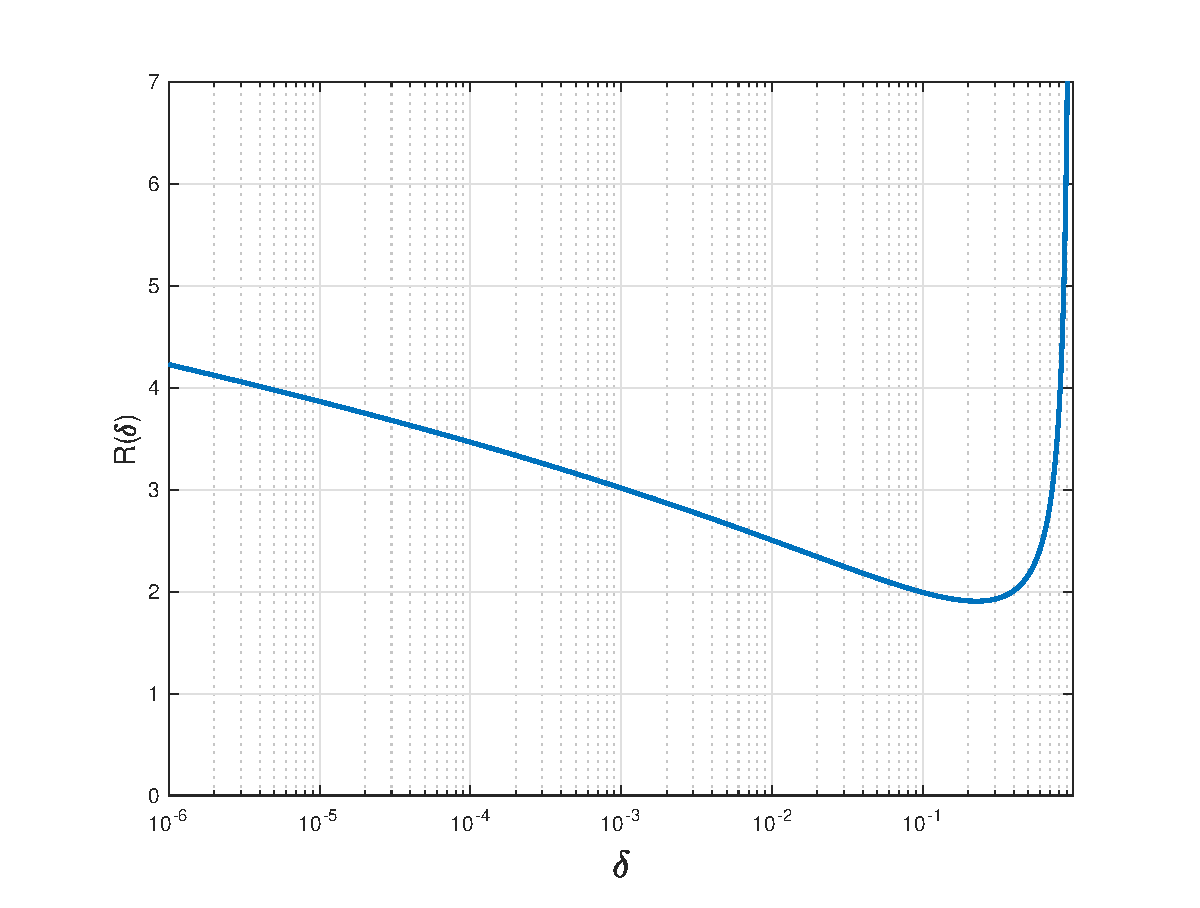
\includegraphics[width = 1.5in]{images/fig_1}\label{fig_1}} \hfil \subfigure[low privacy regime]{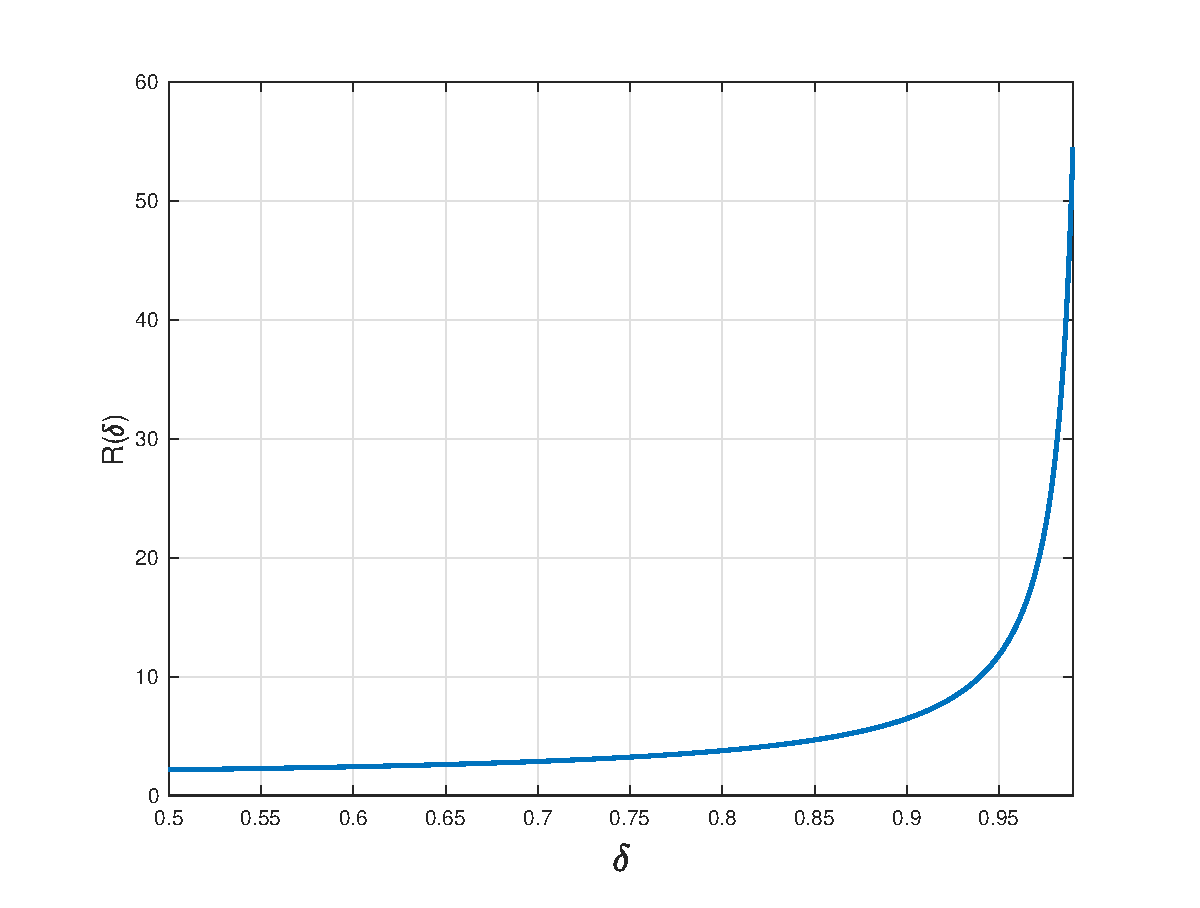
\includegraphics[width = 1.5in]{images/fig_2}\label{fig_2}} }
%\caption{Ratio of expected noise magnitude of the classical Gaussian mechanism to that of proposed mechanism, $ R(\delta)$, plotted against $\delta$.}
%\label{fig_1_2}
%\end{figure} 
%Fig.~\ref{fig_1_2} displays the plot of $ R(\delta)$ against $\delta$. Following inferences could be made from Fig.~\ref{fig_1_2}:
%\begin{itemize}
%\item $R(\delta) > 1$, for all $\delta$ values, indicates that it is not possible for Gaussian mechanism to result in an expected value of noise magnitude less than that of proposed mechanism. 
%\item A multi-fold multiplicative gain, up to several tens in low privacy regime (i.e. high $\delta$), is achieved. 
%\item The gain is high in the high privacy regime, decreases initially with an increasing $\delta$, and finally increases with an increasing $\delta$ in the low privacy regime.            
%\end{itemize}        
%\subsubsection{A Deep Fuzzy Model}
%A deep model, formed by a composition of a finite number of Takagi-Sugeno fuzzy filters, is considered. We consider a particular configuration of the deep fuzzy model, referred to as \emph{deep fuzzy autoencoder}, for data representation learning. 

%Consider a fuzzy filter $(\mathcal{F}: \mathbb{R}^n \rightarrow \mathbb{R})$ that maps $n-$dimensional real-space to a $1-$dimensional real-line. We consider a particular form of Takagi-Sugeno filter where $M$ different $n-$dimensional fuzzy sets are defined on the input space, and corresponding to each fuzzy set, there exists a fuzzy rule of the following type
%\[\begin{array}{ccc}
%\mbox{$m-$th rule} & : & \mbox{If $x$ is $\mathbf{A}^n_m$, then $\mathcal{F}(x) = c_m$}
%\end{array}
%\]            
%where $x  =  \left[\begin{IEEEeqnarraybox*}[][c]{,c/c/c,}x_1 & \cdots & x_n \end{IEEEeqnarraybox*} \right]^T \in \mathbb{R}^n$, $ c_m \in \mathbb{R}$, $m \in \{1,2,\cdots,M\}$, and the fuzzy set $\mathbf{A}^n_m$ is defined, without loss of generality, with the following Gaussian membership function
%\begin{equation}
%\label{eq_Gaussian_multivariate_membership_function}
%\mu_{\mathbf{A}^n_m}(x) = \exp(- \frac{1}{2} \left \|x - a^m  \right \|^2_{W})
%\end{equation}
%where $a^m \in \mathbb{R}^n$ is the mean of $\mathbf{A}^n_m$, $W \in \mathbb{R}^{n \times n} (W > 0)$, and $\left  \| x\right \|^2_{ P} \overset{\underset{\mathrm{def}}{}}{=}  x^TPx$. The output of the filter to input vector $x$ is computed by taking the weighted average of the output provided by each rule, i.e., 
%\begin{IEEEeqnarray}{rCl}
%\label{eq_output_TS_filter}
%\mathcal{F}(x) & = & \frac{\sum_{m = 1}^M \mu_{\mathbf{A}^n_m}(x) c_m}{\sum_{m = 1}^M %\mu_{\mathbf{A}^n_m}(x)}.
%\end{IEEEeqnarray} 
%\begin{definition}[Stochastic Fuzzy Model (SFM)]\label{def_SFM}
%A stochastic fuzzy model, $\mathcal{G}:\mathbb{R}^n \rightarrow \mathbb{R}^p$, maps an input vector $x \in \mathbb{R}^n$ to the output vector $\mathcal{G}(x) \in \mathbb{R}^p$ given as
% \begin{equation}
%\label{eq_FM_output}
%\mathcal{G}(x) = \left[\begin{IEEEeqnarraybox*}[][c]{,c/c/c,}\mathcal{F}_1(x) & \cdots & \mathcal{F}_p(x) \end{IEEEeqnarraybox*} \right]^T \in \mathbb{R}^p
%\end{equation}
%where $\mathcal{F}_j$ ($j \in \{1,2,\cdots, p\}$) is a Takagi-Sugeno fuzzy filter, with consequent parameters being considered as \textbf{random variables} and being represented by a \textbf{random vector} $\alpha_j  =  \left[\begin{IEEEeqnarraybox*}[][c]{,c/c/c,}c_{j,1} & \cdots & c_{j,M} \end{IEEEeqnarraybox*} \right]^T \in \mathbb{R}^M$, such that
%\begin{IEEEeqnarray}{rCl}
%\mathcal{F}_j(x) & = & \frac{\sum_{m = 1}^M \mu_{\mathbf{A}^n_m}(x) c_{j,m}}{\sum_{m = 1}^M \mu_{\mathbf{A}^n_m}(x)}.
%\end{IEEEeqnarray} 
%\end{definition}
%\begin{definition}[Deep Stochastic Fuzzy Model (DSFM)]\label{def_DSFM}
%A deep stochastic fuzzy model, $\mathcal{D}:\mathbb{R}^n \rightarrow \mathbb{R}^p$, maps an input vector $x \in \mathbb{R}^n$ to $\mathcal{D}(x) \in \mathbb{R}^p$ such that
% \begin{IEEEeqnarray}{rCl} 
%\mathcal{D}(x) &=& \mathcal{G}_L\left(\cdots V_3^T\text{E}\left(\mathcal{G}_2\left(V_2^T\text{E}\left(\mathcal{G}_1(V_1^T x)\right)\right)\right)\cdots\right)
% \end{IEEEeqnarray} 
%where $V_1 \in \mathbb{R}^{n \times n_1}, V_2 \in \mathbb{R}^{p \times n_2},\cdots,V_L \in \mathbb{R}^{p \times n_L}$ are some deterministic matrices meant to achieve a lower-dimensional encoding; $\mathcal{G}_l: \mathbb{R}^{n_l} \rightarrow \mathbb{R}^{p}$ ($ l \in \{1,\cdots,L\}$) is a SFM (Definition~\ref{def_SFM}); $\text{E}(\cdot)$ is the expectation; and $L  \in \mathbb{Z}_{+}$ is the number of layers. That is, DSFM processes an input vector through a composition of a finite number of stochastic fuzzy models. 
%\end{definition}
%\begin{definition}[Deep Stochastic Fuzzy Autoencoder]\label{def_DSFAE}
%A deep stochastic fuzzy encoder, $\mathcal{AE}:\mathbb{R}^p \rightarrow \mathbb{R}^p$, maps a vector $y \in \mathbb{R}^p$ to $\mathcal{AE}(y) \in \mathbb{R}^p$ such that
% \begin{IEEEeqnarray}{rCl} 
%y & \approx &  \mathcal{AE}(y) \\
% & \overset{\underset{\mathrm{def}}{}}{=}  &  \mathcal{D}(y),
% \end{IEEEeqnarray} 
%where $\mathcal{D}$ is a DSFM (Definition~\ref{def_DSFM}). 
% \end{definition}
%\subsubsection{Variational Bayesian Inference of Deep Stochastic Fuzzy Autoencoder}
%Variational Bayes, a widely used Bayesian inference method, is applied for the learning of deep fuzzy autoencoder. The standard variational Bayes method \cite{5447695} can be applied for the learning of the deep stochastic fuzzy autoencoder, i.e.,  \begin{IEEEeqnarray}{rCl}
%\label{eq_learning_autoencoder}\mathcal{M} & = & \text{VariationalBayesDeepAutoencoder}\left(\mathrm{Y} \right) 
%\end{IEEEeqnarray}
%where $\text{VariationalBayesDeepAutoencoder}(\mathrm{Y})$ represents the variational Bayes algorithm learning from data matrix $\mathrm{Y}$ for the given priori distributions on model variables and $\mathcal{M}$ is the set of parameters describing the inferred posterior distributions on variables related to autoencoder.
%\subsubsection{Private Deep Stochastic Fuzzy Autoencoder}
%Assuming that the data matrix $\mathrm{Y}$ is private, the deep fuzzy autoencoder is learned in private setting as follows:
%\begin{IEEEeqnarray}{rCl}
%\label{eq_learning_autoencoder_DP} \mathcal{M}^+ & = & \text{VariationalBayesDeepAutoencoder}\left(\mathrm{Y} + \mathrm{V} \right)
%\IEEEeqnarraynumspace
%\end{IEEEeqnarray}  
%where $\mathrm{V}$ is a random noise matrix with $f_{\mathrm{v}_j^i}^*(v)$ being the probability density function of its $(j,i)-$th element given by (\ref{eq_optimal_density_epsilon_delta_privacy}).
%\begin{definition}[Fuzzy Set Induced by Private Autoencoder]\label{def_membership_induced_DFAE}
%Given a private autoencoder $\mathcal{M}^+$, learned as in~(\ref{eq_learning_autoencoder_DP}), a fuzzy set $\mathbf{A}_{\mathcal{M}^+}^p \subset \mathbb{R}^p$ can be defined with e.g. a Gaussian membership function given as  
%\begin{IEEEeqnarray}{rCl}
%\label{eq_membership_function_induced_DFAE} \mu_{\mathbf{A}_{\mathcal{M}^+}^p}\left(y^*\right)  & =  & \exp(- \frac{1}{2p} \left \|y^* -  \hat{y}^{*} \right \|^2 ),
%\end{IEEEeqnarray}
%where $\hat{y}^{*}$ is expected output of the autoencoder corresponding to input $y^* \in \mathbb{R}^p$. 
%\end{definition} 
%\subsubsection{Differentially Private Distributed Learning for Classification}
%An application to data classification problems is possible via learning through deep fuzzy autoencoder a representation of the given training samples of a particular class. Assume that there are $S$ different datasets, $\mathrm{Y}^1,\cdots,\mathrm{Y}^S$, owned locally by $S$ different participants. We study specifically the data classification problem assuming that each local dataset, say $\mathrm{Y}^s$, can be partitioned into $C$ different classes, i.e.,
%\begin{IEEEeqnarray}{rCl}
%\mathrm{Y}^s &= & \{\mathrm{Y}^s_1,\cdots,\mathrm{Y}^s_C \} 
%\end{IEEEeqnarray}
%where $\mathrm{Y}^s_c$ refers to the datamatrix corresponding to $c-$th class owned locally by $s-$th participant. Let $\mathcal{M}^{+s}_c$ be the deep fuzzy autoencoder learned using $\mathrm{Y}^s_c$ in the private setting. As per Definition~\ref{def_membership_induced_DFAE}, a fuzzy set $\mathbf{A}_{\mathcal{M}^{+s}_c}^p \subset \mathbb{R}^p$ is induced by $\mathcal{M}^{+s}_c$.

%The post-processing invariance property of differential privacy allows to compose a global private fuzzy classifier from local private deep autoencoders. We suggest a global fuzzy classifier based on following if-then fuzzy rules:
% \begin{IEEEeqnarray}{CCl}
%\nonumber \mbox{If $y^*$ is $\mathbf{A}_{\mathcal{M}^{+1}_1}^p$ OR $\mathbf{A}_{\mathcal{M}^{+2}_1}^p$ OR $\cdots$ OR $\mathbf{A}_{\mathcal{M}^{+S}_1}^p$,}  \\
%\nonumber \mbox{then the class is $1$}; \\
%\label{eq_fuzzy_rules_classification} \vdots & &  \\
%\nonumber \mbox{If $y^*$ is $\mathbf{A}_{\mathcal{M}^{+1}_C}^p$ OR $\mathbf{A}_{\mathcal{M}^{+2}_C}^p$ OR $\cdots$ OR $\mathbf{A}_{\mathcal{M}^{+S}_C}^p$,}  \\
%\nonumber \mbox{then the class is $C$}. 
%\end{IEEEeqnarray} 
%The label associated to a new data point $y^*$ is predicted based on fuzzy rules~(\ref{eq_fuzzy_rules_classification}) as
%\begin{IEEEeqnarray}{rCl}
%c^{*} & = & \arg \; \max_{\displaystyle 1 \leq c \leq C} \; \left( \max_{\displaystyle 1 \leq s \leq S} \;\mu_{\mathbf{A}_{\mathcal{M}^{+s}_c}^p}\left(y^*\right) \right)
%\end{IEEEeqnarray} 
%where $\mu_{\mathbf{A}_{\mathcal{M}^{+s}_c}^p}\left(y^*\right)$ is the membership value computed using (\ref{eq_membership_function_induced_DFAE}).

%\begin{figure}[!h]
%\centering
 %\scalebox{0.75}{
 %\begin{tikzpicture}[multilayer = 3d]
%\SetLayerDistance{2}
%\Plane[x=0,y=0,width=4,height=2,RGB,color={235,235,235},InBG=True,NoBorder=True,layer=1]
%\Vertex[size=1,x=1,y=1,label=$\mathrm{Y}^1$,fontscale=1,layer=1]{y}
%\Vertex[size=1,x=3,y=1,label=$\mathrm{Y}^2$,fontscale=1,layer=1,color=orange!50!white]{y2}
%\Plane[x=0,y=0,width=4,height=2,RGB,color={255,184,184},InBG=True,NoBorder=True,layer=2]
%\Vertex[size=1,x=1,y=1,label=$\mathrm{Y}^{+1}$,fontscale=1,layer=2]{y+}
%\Vertex[size=1,x=3,y=1,label=$\mathrm{Y}^{+2}$,fontscale=1,layer=2,color=orange!50!white]{y2+}
%\Edge[color=blue,lw=1,bend=0](y+)(y)
%\Edge[color=blue,lw=1,bend=0,color=orange](y2+)(y2)
%\Plane[x=0,y=0,width=4,height=2,RGB,color={235,235,235},InBG=True,NoBorder=True,layer=3]
%\Vertex[size=1.5,x=1,y=1,label=$\{\mathcal{M}_c^{+1}\}_{c=1}^C$,fontscale=1,layer=3,color=red!30!white]{M}
%\Vertex[size=1.5,x=3,y=1,label=$\{\mathcal{M}_c^{+2}\}_{c=1}^C$,fontscale=1,layer=3,color=red!30!white]{M2}
%\Edge[color=red,lw=1,bend=0](y+)(M)
%\Edge[color=red,lw=1,bend=0](y2+)(M2)
%\Plane[x=0,y=0,width=4,height=2,RGB,color={235,235,235},InBG=True,NoBorder=True,layer=4]
%\Vertex[size=1.75,x=2,y=1,label=fuzzy rules~(\ref{eq_fuzzy_rules_classification}),fontscale=1,layer=4,color=red!30!white]{fuzzy_rules}
%\Edge[color=blue,lw=1,bend=0,color=red](M)(fuzzy_rules)
%\Edge[color=blue,lw=1,bend=0,color=red](M2)(fuzzy_rules)
%\Text[x=3.75,y=1.8,style={draw,rectangle},fontsize=\small,layer=1]{1.}
%\Text[x=5.1,y=1.8,style={color=blue},width=2cm,fontsize=\small,layer=1]{local data}
%\Text[x=3.75,y=1.8,style={draw,rectangle},fontsize=\small,layer=2]{2.}
%\Text[x=6.1,y=1.60,style={color=blue},width=4cm,fontsize=\small,layer=2]{privacy wall $(\epsilon,\delta)-$differential privacy}
%\Text[x=3.75,y=1.8,style={draw,rectangle},fontsize=\small,layer=3]{3.}
%\Text[x=5.35,y=1.6,style={color=blue},width=2.5cm,fontsize=\small,layer=3]{local private deep models}
%\Text[x=3.75,y=1.8,style={draw,rectangle},fontsize=\small,layer=4]{4.}
%\Text[x=5.35,y=1.6,style={color=blue},width=2.5cm,fontsize=\small,layer=4]{global fuzzy classifier}
%\end{tikzpicture}
%}
%\caption{A structural representation of the differentially private distributed learning for classification.}
%\label{fig_structural_representation_distributed_differential_private}
%\end{figure} 
%The distributed form of differentially private learning of a fuzzy classifier is represented in Fig.~\ref{fig_structural_representation_distributed_differential_private} where a privacy wall is inserted between training data and the globally shared data. The privacy wall uses noise adding mechanisms to attain differential privacy for each participant's private training data. Therefore, the adversaries have no direct access to the training data. 
     



